\documentclass{article}

% https://tex.stackexchange.com/questions/106988/package-for-drawing-rdf-graphs

\title{
Distributed AMIE+\\
\large Preliminary Notes\\
of the Thesis Project\\
}
\author{Omar Trinidad Guti\'errez M\'endez}

\usepackage{amsmath}
\usepackage[utf8]{inputenc}
\usepackage{amsmath}
\usepackage{graphicx}
\usepackage{xcolor}
%\usepackage{venndiagram}

% Tikz section %%%%%%%%%%%%%%%%%%%%%%%%%%%%%%%%%%%%%%%%%%%%%%%%%%%%%%%%%%%%%%%%

\usepackage{tikz}
    \usetikzlibrary{shapes.geometric, backgrounds, calc}
    \usetikzlibrary{arrows}
    \usetikzlibrary{positioning}
    \usetikzlibrary{chains}

% For every picture that defines or uses external nodes, you'll have to
% apply the 'remember picture' style. To avoid some typing, we'll apply
% the style to all pictures.
\tikzstyle{every picture}+=[remember picture]

% By default all math in TikZ nodes are set in inline mode. Change this to
% displaystyle so that we don't get small fractions.
\everymath{\displaystyle}

% Tikz section %%%%%%%%%%%%%%%%%%%%%%%%%%%%%%%%%%%%%%%%%%%%%%%%%%%%%%%%%%%%%%%%

\begin{document}
\maketitle

\section{Introduction}

Knowledge bases (KB) have the purpose of representing and store knowledge in a
machine-readable format. Some well-known KBs are DBpedia~\cite{dbpedia-swj},
NELL, YAGO~\cite{suchanek2007yago}, or Freebase~\cite{bollacker2008freebase}. A
usual task executed in these databases is mining logical rules, that is, find
unknown relationships between entities.

However,  these databases are designed under the idea of Open World Assumption
(OWA), that means, if the database does not contain a fact, we are not assuming
that this fact is false, as happens under the Closed World Assumption (CWA).

Finding these relations in huge datasets, and under the OWA setting is a
challenging task. This problem was addressed by Galárraga et
al.~\cite{galarraga2013amie}  who proposed Association Rule Mining under
Incomplete Evidence (AMIE) and later suggested an improved version of the same
method that they simple named AMIE+~\cite{galarraga2015fast}.

The purpose of the current project is to explore AMIE+ and implement it in a
distributed context.

\subsection{Theoretical framework}

%~\cite{rdf}
Knowledge Bases $KB$ are collections of facts; every fact is represented by a
relation between a subject and object $r(s, o)$. In this work, we are focused
on KBs modeled using the W3C standard Resource Description Framework
(RDF). In RDF, the facts are represented as triples.


An \textit{atom} is a fact with variables at the subject and/or object. A Horn
rule is composed of a head and a body.

\begin{itemize}
    \item The head is a single atom \tikz\node [fill=green!20,draw,circle] (n3) {};
    \item The body is a set of atoms \tikz\node [fill=blue!20,draw,circle] (n1) {};
\end{itemize}

% Below we mix an ordinary equation with TikZ nodes
\begin{equation}
        \tikz[baseline]{
            \node[fill=blue!20,anchor=base] (b1)
            { $B_1$ };
        } \land
        \tikz[baseline]{
            \node[fill=blue!20,anchor=base] (b2)
            { $B_2$ };
        } \land \ldots \land
        \tikz[baseline]{
            \node[fill=blue!20,anchor=base] (b3)
            { $B_n$ };
        }
        \implies
        \tikz[baseline]{
            \node[fill=green!20,anchor=base] (head)
            { $r(x, y)$ };
        }
\end{equation}

% Draw some edges between the global nodes
\begin{tikzpicture}[overlay]
        \path[->] (n1) edge [out=-100, in=-250] (b1);
        \path[->] (n1) edge [out=-100, in=-250] (b2);
        \path[->] (n1) edge [out=-100, in=-250] (b3);
        \path[->] (n3) edge [out=0, in=-250] (head);
\end{tikzpicture}

% ¿Es relevante?
% The facts in KBs are divided in A-Box and T-Box.

\subsubsection{Horn rules and language bias}

In order to limit the size of the search space, AMIE uses constraints that are called
\textit{language bias}.

% ToDo
% Tikz figure showing examples of rules.
% Tikz figures for SANSA stack.

There is an aim to limit the size of the search space, with AMIE, for example,
we use constraints on the structure of the mined rules, this is called language
bias. The idea is to have good designed language bias to avoid to deal with an
intractable search space but at the same time to generate more expressive rules.

\begin{itemize}
    \item We aim for connectivity, two atoms in a rule are connected if they share a variable or
entity. A rule is connected when every atom is connected transitively to the
rest of atoms.
    \item The rules have to be closed.
    \item Also, reflexive rules are discarded.
\end{itemize}

\subsubsection{Measures of significance}

We want to use only rules above a given support threshold.

\subsubsection{Incompleteness}

As was stated before, the semantic KBs operate under the CWA, that is, we
assume the facts in the database are known true facts, everything else, outside
the database is asumed to be unknown.

Going beyond, we say that the unknown facts are either true or false facts, we
want to predict the new ones.

\begin{figure}
\resizebox{7.555cm}{!}{%
    
% for drawing
\def\firstellip{(0, 0) ellipse [x radius=3cm, y radius=3cm, rotate=50]}
\def\bounding{(-5,-3) rectangle (5,4)}

\begin{tikzpicture}

    \filldraw[fill=black, opacity=0.2] \bounding;

    %\scope \fill[white] \fourthellip; \endscope \filldraw[fill=red, opacity=0.2] \fourthellip;

    %single colors
    \scope
        \fill[white] \firstellip;
    \endscope

    \draw \firstellip node [label={[xshift=1.333cm, yshift=0.999cm]All here is true}] {};
    \draw \firstellip node [label={[xshift=1.333cm, yshift=2.999cm]All here is unknown}] {};

   % \draw \secondellip node [label={[xshift=2.2cm, yshift=2.1cm]$B$}] {};
   % \draw \thirdellip node [label={[xshift=-2.0cm, yshift=-0.9cm]$C$}] {};
   % \draw \fourthellip node [label={[xshift=-2.2cm, yshift=2.1cm]$D$}] {};
     \draw \bounding node [label=above left:$U$] {};

   % \begin{scope}
   %     \begin{scope}[even odd rule]% first ellipse corner
   %         \clip \secondellip (-5,-5) rectangle (5,5);
   %         \clip \thirdellip (-5,-5) rectangle (5,5);
   %         \clip \fourthellip (-5,-5) rectangle (5,5);
   %     \fill[yellow] \firstellip;
   %     \end{scope}
   % \end{scope}

   % \begin{scope}
   %     \begin{scope}[even odd rule]% second ellipse corner
   %         \clip \firstellip (-5,-5) rectangle (5,5);
   %         \clip \thirdellip (-5,-5) rectangle (5,5);
   %         \clip \fourthellip (-5,-5) rectangle (5,5);
   %     \fill[yellow] \secondellip;
   %     \end{scope}
   % \end{scope}

   % \begin{scope}
   %     \begin{scope}[even odd rule]% third ellipse corner
   %         \clip \secondellip (-5,-5) rectangle (5,5);
   %         \clip \firstellip (-5,-5) rectangle (5,5);
   %         \clip \fourthellip (-5,-5) rectangle (5,5);
   %     \fill[yellow] \thirdellip;
   %     \end{scope}
   % \end{scope}

\end{tikzpicture}

}
\caption{Flowchart of AMIE algorithm}
\label{fig:kb}
\end{figure}

\subsection{Similar works}

The task of finding new logical rules given a KB has been addressed from
multiple angles. For example, ILP based approaches, relational machine learning
or hybrid approaches.

One advantage, from AMIE over relational machine learning approaches, is that
AMIE has better interpretability, which is a crucial in the Data Science world.
So, with AMIE, it is possible to mine logical rules where there is a
correlation in the data.

\subsection{AMIE}

% The purpose of AMIE is to generate Horn rules.

Inside AMIE, the Partial Completeness Assumption (PCA) was used to guess the
so-called counterexamples for rules.

In the PCA we say that a subject-relation pair is complete if it does exists
an object that for that s,r.

Assume that if the KB knows relations for some subject then knows all the set
of values.

%\subsubsection{Completeness}
%Lets say that $KB*$ contains every fact of the world.

\subsection{AMIE plus}

\begin{figure}[htbp]
\resizebox{!}{18cm}{%
    % -------------------------------------------------
% Set up a new layer for the debugging marks, and make sure it is on
% top
% this is a good example: https://tex.stackexchange.com/questions/254136/how-do-i-fix-spacing-on-paths-for-a-nested-tikz-flowchart

\pgfdeclarelayer{marx}
\pgfsetlayers{main,marx}
% A macro for marking coordinates (specific to the coordinate naming
% scheme used here). Swap the following 2 definitions to deactivate
% marks.
\providecommand{\cmark}[2][]{%
  \begin{pgfonlayer}{marx}
    \node [nmark] at (c#2#1) {#2};
  \end{pgfonlayer}{marx}
  } 
\providecommand{\cmark}[2][]{\relax} 
% -------------------------------------------------

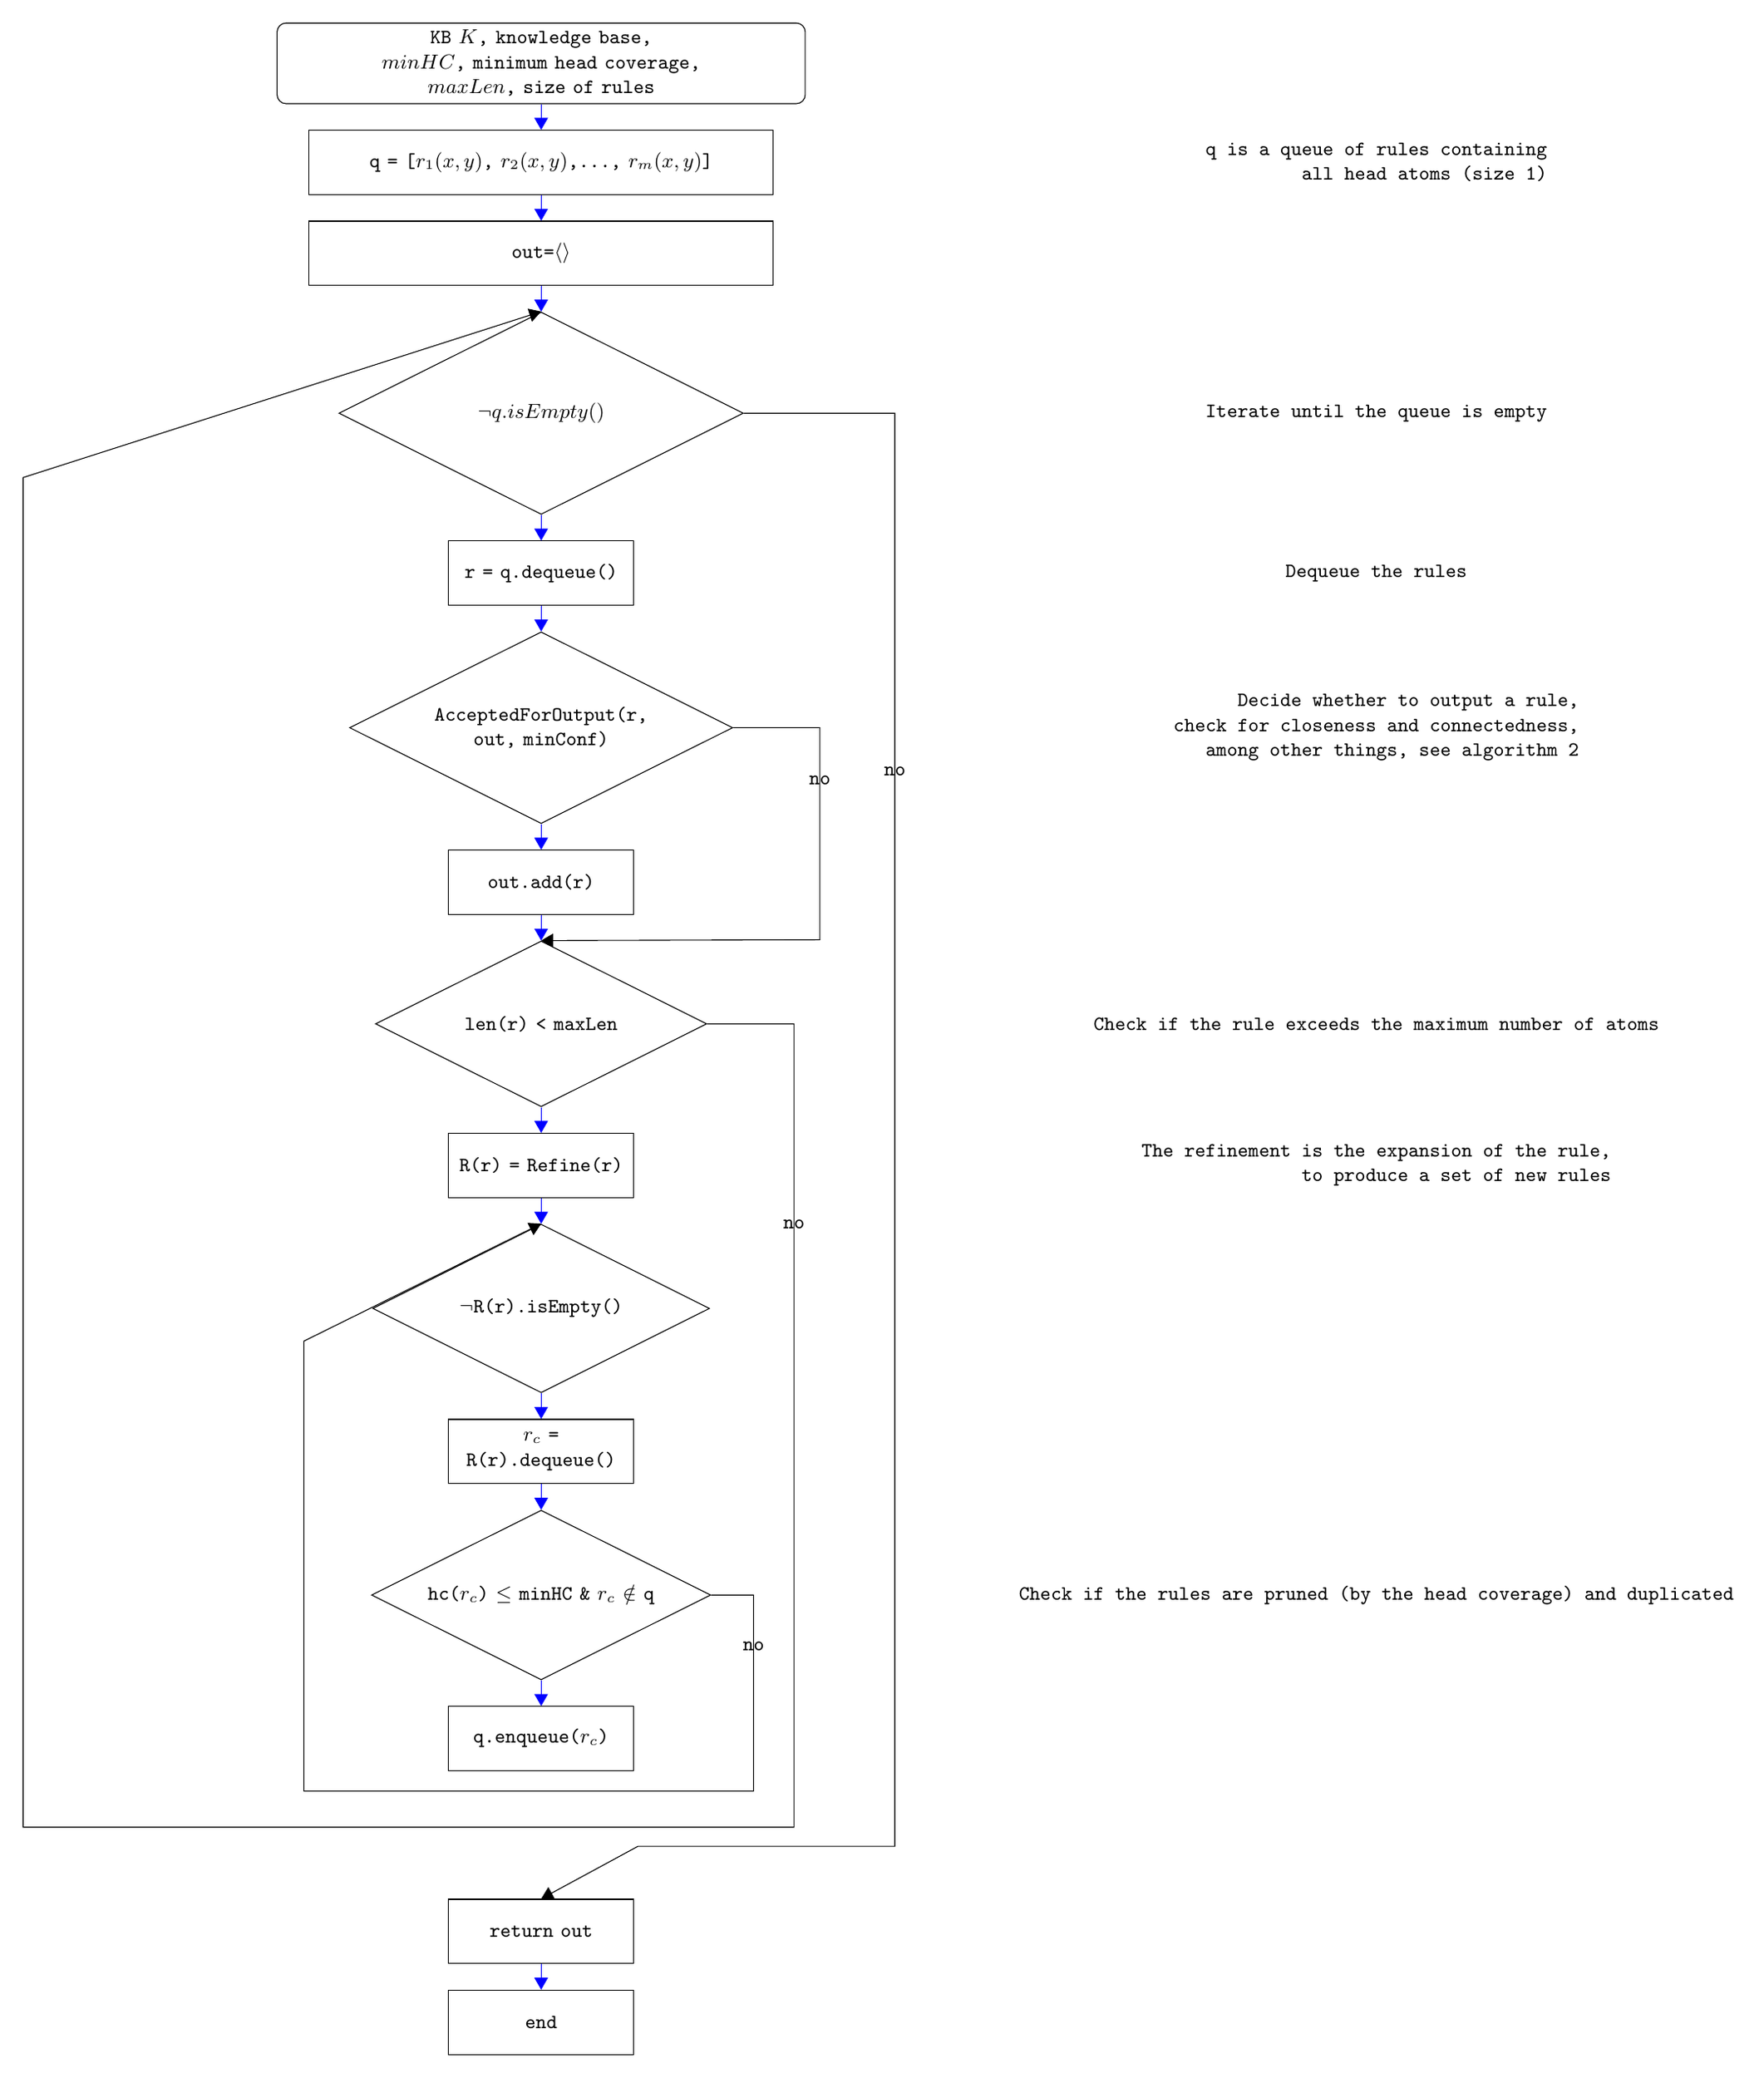
\begin{tikzpicture}[%
    >=triangle 60,              % Nice arrows; your taste may be different
    start chain=going below,    % General flow is top-to-bottom
    node distance=4mm and 10mm, % Global setup of box spacing
    every join/.style={norm},   % Default linetype for connecting boxes
    ]

{\small\ttfamily\selectfont
% ------------------------------------------------- 
% A few box styles 
% <on chain> *and* <on grid> reduce the need for manual relative
% positioning of nodes
\tikzset{
  base/.style={draw, on chain, on grid, align=center, minimum height=1cm, font={\small}},
  notes/.style={node distance=13cm, align=right},
  diam/.style={base, diamond, aspect=2, text width=5cm},
  diam_small/.style={base, diamond, aspect=2, text width=4cm},
  proc/.style={base, rectangle, text width=7cm},
  proc_small/.style={base, rectangle, text width=8em},
  term/.style={proc, rounded corners, text width=8cm},
  % coord node style is used for placing corners of connecting lines
  coord/.style={coordinate, on chain, on grid, node distance=6mm and 15mm},
  % nmark node style is used for coordinate debugging marks
  nmark/.style={draw, cyan, circle, font={\sffamily\bfseries}},
  % -------------------------------------------------
  % Connector line styles for different parts of the diagram
  norm/.style={->, draw, blue},
  free/.style={->, draw, green},
  cong/.style={->, draw, red},
  it/.style={font={\small\itshape}}
}
% -------------------------------------------------
% Start by placing the nodes
% Use join to connect a node to the previous one a

\node [term] (p0) {
    KB $K$, knowledge base,\\
    $minHC$, minimum head coverage,\\
    $maxLen$, size of rules
};
\node [proc, join] (q) {
    q = [$r_1(x, y)$, $r_2(x, y)$,\ldots, $r_m(x,y)$]
};
\node [proc, join] (p2) {
    out=$\langle\rangle$
};
\node [diam, join] (is_empty) {
    $\lnot q.isEmpty()$
};
\node [proc_small, join] (dequeue) {
    r = q.dequeue()
};
\node [diam_small, font={\small}, join] (accepted_for_output) {
    AcceptedForOutput(r, out, minConf)
};
\node [proc_small, join] (p6) {
    out.add(r)
};
\node [diam_small, join] (check_max_len) {
    len(r) < maxLen
};
\node [proc_small, join] (refinement) {
    R(r) = Refine(r)
};
\node [diam_small, join] (p9) {
    $\lnot$R(r).isEmpty()
};
\node [proc_small, join] (dequeue_refinement) {
    $r_c$ = R(r).dequeue()\\
};
\node [diam_small, join] (check) {
    hc($r_c$) $\leq$ minHC \& $r_c$ $\notin$ q
};
\node [proc_small, join] (p11) {
    q.enqueue($r_c$)
};
\node [proc_small, below of = p11, node distance = 2.6cm] (return) {return out};
\node [proc_small, join] (end) {end};


\draw[->] (check.east) -- ++(0.66,0) -- ++(0,-0.05) -- node [near start] {no} ++(0,-3.0) -- ++(-7,0) -- ++(0, 7) -- (p9.north);
\draw[->] (is_empty.east)  -- ++(0,0.0) -- ++(2.35,0) -- node [near start] {no} ++(0,-22.3) -- ++(-4,0) -- (return.north);
\draw[->] (accepted_for_output.east)  -- ++(0,0.0) -- ++(1.35,0) -- node [near start] {no} ++(0,-3.3) -- (check_max_len.north);
\draw[->] (check_max_len.east)  -- ++(0,0.0) -- ++(1.35,0) -- node [near start] {no} ++(0, -12.5) -- ++(-12,0) -- ++(0, 21) -- (is_empty.north);

% notes
\node [notes, right of=q] {q is a queue of rules containing\\all head atoms (size 1)};
\node [notes, right of=is_empty] {Iterate until the queue is empty};
\node [notes, right of=refinement] {The refinement is the expansion of the rule,\\to produce a set of new rules};
\node [notes, right of=dequeue] {Dequeue the rules};
\node [notes, right of=accepted_for_output] {Decide whether to output a rule,\\check for closeness and connectedness,\\among other things, see algorithm 2};
\node [notes, right of=check] {Check if the rules are pruned (by the head coverage) and duplicated};
\node [notes, right of=check_max_len] {Check if the rule exceeds the maximum number of atoms};

}
\end{tikzpicture}

}
\caption{Flowchart of AMIE algorithm}
\label{fig:amie_flowchart}
\end{figure}

In AMIE+ it was aggregated pruning strategies and approximations that allowed
to explore the search space more efficiently.

\subsection{SANSA Stack}

SANSA~\cite{lehmann-2017-sansa-iswc} is a platform whose purpose is\ldots

\bibliographystyle{plain}
\bibliography{notes}

\end{document}
